\chapter{Distributional Semantics}
\label{sec:background}

\section{Chapter Overview}

In this section, we review some of the background critical to this proposal.
We begin with a discussion of Recognizing Textual Entailment and the core
motivation of our thesis.  We then overview Distributional Semantics, outlining
its purpose and one common implementation of VSMs. Finally, we discuss the
Lexical Entailment (LexEnt) and Lexical Substitution (LexSub) tasks, which we
view as two useful proxies for the kinds of lexical semantics necessary in
RTE. We do not argue that these tasks are completely sufficient, but one goal
of our thesis to show that developments in these tasks improves practical RTE.

\section{Background: Distributional Semantics}
\label{sec:dist}

Distributional Semantics is a powerful tool for automatically inducing semantic
representations for lexical items \cite{turney:2010:jair,erk:2012:llc}.  The
core notion is that of the {\em Distributional Hypothesis}, that if two words
appear in similar {\em contexts}, they can be assumed to have similar meaning.
This idea has a long history in the linguistic and philosophical literature that
can be traced back over 60 years
\cite{wittgenstein:1953:pi,harris:1954:word,firth:1957:la}. In its modern form,
Distributional Semantics involves finding {\em vector space representations} of
words which are constructed by counting or modeling the contexts in which a
particular word appears. According to the Distributional Hypothesis, words
with similar {\em vectors} can be assumed to have similar {\em meanings}
\cite{turney:2010:jair}. For this reason, they are often referred to as
Vector Space Models (VSMs) of language. Variations on this idea have also
become immensely popular in the neural networks community, with algorithms
like Skip-gram Negative Sampling (SGNS) \cite{mikolov:2013:iclr} and GloVe
\cite{pennington:2014:emnlp}, and have often replaced traditional count-based
VSMs in the NLP community \cite{baroni:2014:acl}.

\begin{figure}
\centering
\begin{minipage}{7cm}
\begin{scriptsize}
\begin{alltt}
         the furry {\color{TealBlue}{dog}} is friendly to
and manipulate the {\color{TealBlue}{dog}} 's lips and
       as a clever {\color{TealBlue}{dog}} ; two to
a reputation among {\color{TealBlue}{dog}} trainers of having
    also among the {\color{TealBlue}{dog}} breeds most likely
 the very earliest {\color{TealBlue}{dog}} shows and kennel
        as a guard {\color{TealBlue}{dog}} and to hunt
   the mechanic 's {\color{TealBlue}{dog}} began to howl
\end{alltt}
\end{scriptsize}
\end{minipage}
\begin{minipage}{7cm}
\begin{center}
\begin{tikzpicture}[scale=1.3]
    % Draw axes
    \def\r{0.5}
    % Draw two intersecting lines
    \coordinate (origin) at (0,0);
    \coordinate (cat) at ($(origin) + (76:1.7)$);
    \coordinate (dog) at ($(origin) + (66:1.1)$);
    \coordinate (ani) at ($(origin) + (12:2.1)$);

    \draw [->,TealBlue] (origin) -- (dog) node[right] {\word{dog}};
    \draw [->,Purple] (origin) -- (cat) node[right] {\word{cat}};
    \draw [->,Green] (origin) -- (ani) node[right] {\word{animal}};

    \draw [] (12:\r) arc (12:66:\r) node[right,pos=0.75] {$\theta$};
    \draw [->,line width=0.3mm] (origin) -- (0,2) node (yaxis) [above,pos=0.5,rotate=90] {{ furry}};
    \draw [->,line width=0.3mm] (origin) -- (3,0) node (xaxis) [below,pos=0.5] {{ underwater}};

\end{tikzpicture}
\end{center}
\end{minipage}
\caption{(a) Example contexts of the word \word{dog}, and (b) cartoon drawing
of word vectors in the \word{furry} and \word{underwater} dimensions.}
\label{fig:vsm}
\end{figure}

In its simplest form, vectors are induced by defining a vector space where
each dimension in the space corresponds to a particular context word. A large,
unannotated corpus of text is then processed, finding instances of a target word,
like {\em dog}, and incrementing a count for each of the target's {\em
co-occurrences}, or words appearing around the target word
{\em dog}, as in Figure~\ref{fig:vsm}. With a large enough corpus, coherent
statistical patterns begin to form. For example, the word {\em furry} is likely
to be used to describe both {\em cat} and {\em dog}, which is then reflected in
the vector counts \cite{lund:1996:brmic}. After constructing vector
representations for the words {\em cat} and {\em dog}, we can then compare
these vectors using various geometric distance metrics, most prominently {\em
cosine similarity}:
\begin{equation}
  \text{cosine}(u, v) = \frac{\sum_i u_iv_i}{\sqrt{\sum_i u_i^2 \sum_i v_i^2}}
  \label{eq:cos}
\end{equation}
Here, $i$ iterates over all the different context dimensions, like {\em furry}
or {\em kennel}, and cosine similarity is defined over the range $[-1, 1]$.
Words with similar vectors will have a smaller angle between them, and therefore
a higher cosine similarity (i.e. close to 1).

\paragraph{Count Transformations}
In practice, usually the distributional vectors are more sophisticated in their
construction than raw co-occurrence counts.  Typically, words and contexts
below a certain threshold are omitted from the co-occurrence matrix, because
extremely rare words have few counts and therefore impoverished representations
\cite{turney:2010:jair}. The co-occurrence matrix is also usually transformed
using some nonlinearity; one common choice is Positive Pointwise Mutual
Information (PPMI) \cite{bullinaria:2007:brm}, where the raw co-occurrence count
between a word $w$ and context $c$ is transformed,
\begin{equation*}
  \text{PPMI}(w, c) = \max\left(0, \log\frac{P(w, c)}{P(w)P(c)}\right)
\end{equation*}
Pointwise Mutual Information (PMI) measures roughly how many times more likely two
items co-occur more often than chance, while Positive PMI
additionally ignores co-occurrences that occur less often than chance.  Other
transformations, like conditional probability
\cite{hofman:1999:sigir,blei:2003:jmlr} and Softplus
\cite{pennington:2014:emnlp}, are also sometimes seen in the literature, and
emphasize different aspects of lexical similarity.

\paragraph{Syntactic Contexts}
Defining contexts is another important aspect of Distributional Semantics.
In the example of Figure~\ref{fig:vsm}, we showed that context can be defined
as three words to the left and right of the target word, but there are
alternatives. For example, using very large windows of co-occurrence (or even
entire documents) results in emphasizing more {\em topical} similarity, e.g. doctor
and hospital, while smaller windows emphasize more {\em functional} similarity, e.g.
doctor and surgeon \cite{pado:2007:cl,erk:2008:emnlp,levy:2014:acl}.

Context can be also defined as {\em syntactic neighbors} extracted from a
dependency parse. For example, in Figure~\ref{fig:syn}, the
contexts for the word {\em chased} would be {\em nsubj+dog} and {\em
dobj+tail}. Distributional Spaces defined in this manner tend to emphasize the
{\em selectional preferences} of words, or the tendency of words to have
particular arguments in their syntactic relations.
\cite{pado:2007:cl,erk:2008:emnlp,baroni:2010:cl,levy:2014:acl}. For example,
the subject of {\em barks} is likely to be {\em dog}, while the subject of
{\em purrs} is likely to be {\em cat}.

\begin{figure}
  \centering
  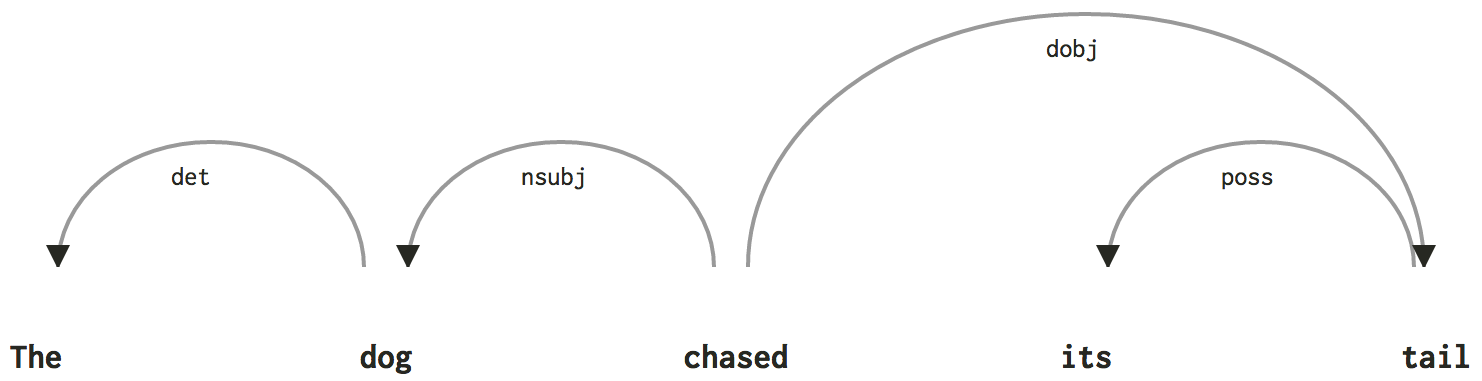
\includegraphics[width=0.75\textwidth]{figures/syn}
\caption{Example of a dependency parse for ``The dog chased its tail.'' In
a syntactic distributional space, contexts are defined as adjacent nodes
with their labeled edges.}
\label{fig:syn}
\end{figure}

\paragraph{Dimensionality Reduction}
Dimensionality Reduction is another important aspect of Distributional Semantics.
As described earlier, distributional vector
spaces are very high-dimensional: bag-of-words spaces have many thousands of
dimensions \cite{turney:2010:jair,mikolov:2013:iclr,pennington:2014:emnlp},
while syntactic spaces usually have a millions \cite{baroni:2010:cl}.
Efficiently dealing with these large, extremely sparse vectors can be
troublesome, so we often opt to use some form of {\em dimensionality
reduction}, like Singular Value Decomposition (SVD)
\cite{deerwester:1990:jsis,landauer:1997:pr} or Nonnegative Matrix
Factorization (NNMF) \cite{lee:2000:nips}. In dimensionality reduction, the
co-occurrence matrix $M$ is typically assumed to be factorizable into two
lower-rank matrices,
\begin{equation}
  M = VC^{\top}
  \label{eqn:svd}
\end{equation}
where $V$ is some lower dimension representation of word vectors, and $C$ is
the corresponding lower dimension representation of the context items. These
projections of words and contexts into the same latent space traces back to the
earliest days of distributional semantics \cite{deerwester:1990:jsis}, and is
critical to many of the contributions of our completed work.  Interestingly,
the most popular algorithms for computing word embeddings, like Skip-Gram
Negative Sampling (SGNS) \cite{mikolov:2013:iclr} and GloVe
\cite{pennington:2014:emnlp} can be viewed as form of dimensionality reduction
\cite{levy:2014:nips,levy:2015:tacl}.

\section{Chapter Summary}

